\documentclass[tikz]{standalone}

\usepackage{fontspec}

\usetikzlibrary{arrows}
\usetikzlibrary{calc}
\usetikzlibrary{decorations.pathreplacing}
\usetikzlibrary{positioning}
\usetikzlibrary{matrix}

\usepackage{fontspec}

\begin{document}

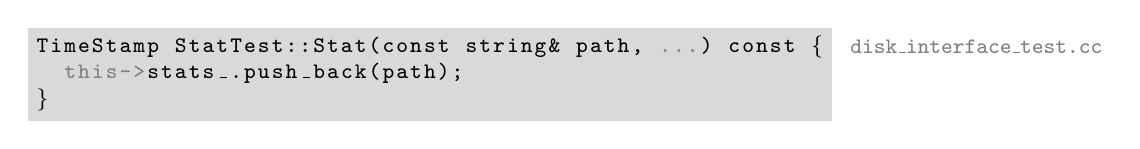
\begin{tikzpicture}
  [node distance=5mm, >=stealth',
  every node/.style={font=\footnotesize},
  every matrix/.style={fill=black!15, inner sep=1mm, row sep=0.5mm,
                        matrix of nodes, nodes in empty cells,
                        minimum height=0.5em, minimum width=.5em,
                        nodes={anchor=base, inner sep=0, font=\ttfamily\footnotesize}}]

  \matrix (snippet) {
T & i & m & e & S & t & a & m & p &   & S & t & a & t & T & e & s & t & : & : & S & t & a & t & ( & c & o & n & s & t &   & s & t & r & i & n & g & \& &   & p & a & t & h & , &   & |[black!50]|. & |[black!50]|. & |[black!50]|. & ) &   & c & o & n & s & t &   & \{ \\
  &   & |[black!50]|t & |[black!50]|h & |[black!50]|i & |[black!50]|s & |[black!50]|- & |[black!50]|> & s & t & a & t & s & \_ & . & p & u & s & h & \_ & b & a & c & k & ( & p & a & t & h & ) & ; &   &   &   &   &   &   &   &   &   &   &   &   &   &   &   &   &   &   &   &   &   &   &   &   &   &   \\
\} &   &   &   &   &   &   &   &   &   &   &   &   &   &   &   &   &   &   &   &   &   &   &   &   &   &   &   &   &   &   &   &   &   &   &   &   &   &   &   &   &   &   &   &   &   &   &   &   &   &   &   &   &   &   &   &   \\
  };

  \node [above, anchor=west, black!50, xshift=2mm]
        at (snippet-1-57.east)
        {\texttt{disk\_interface\_test.cc}};
\end{tikzpicture}

\end{document}
